\documentclass[10pt]{beamer}
\usetheme{Madrid}
\usecolortheme{default}

\usepackage[utf8]{inputenc}
\usepackage{amsmath,amssymb}
\usepackage{algorithm,algorithmicx,algpseudocode}
\usepackage{booktabs}
\usepackage{tikz}

\title[DP-GCD]{High-Dimensional Private Empirical Risk Minimization\\by Greedy Coordinate Descent}
\author{Pierre Cornilleau, \& Amine Belkasmi}
\institute{Differential Privacy in ML project}
\date{March 2026}

\begin{document}

\frame{\titlepage}

\begin{frame}{Outline}
\tableofcontents
\end{frame}

\section{Motivation}

\begin{frame}{The Privacy-Utility Dilemma}
\begin{columns}[T]
\column{0.5\textwidth}
\textbf{Why Privacy Matters}
\begin{itemize}
\item Medical records
\item Financial data
\item Personal information
\item Legal requirements (GDPR)
\end{itemize}

\vspace{1em}
\textbf{The Problem}
\begin{itemize}
\item Models leak training data
\item Membership inference attacks
\item Model inversion attacks
\end{itemize}

\column{0.5\textwidth}
\begin{center}
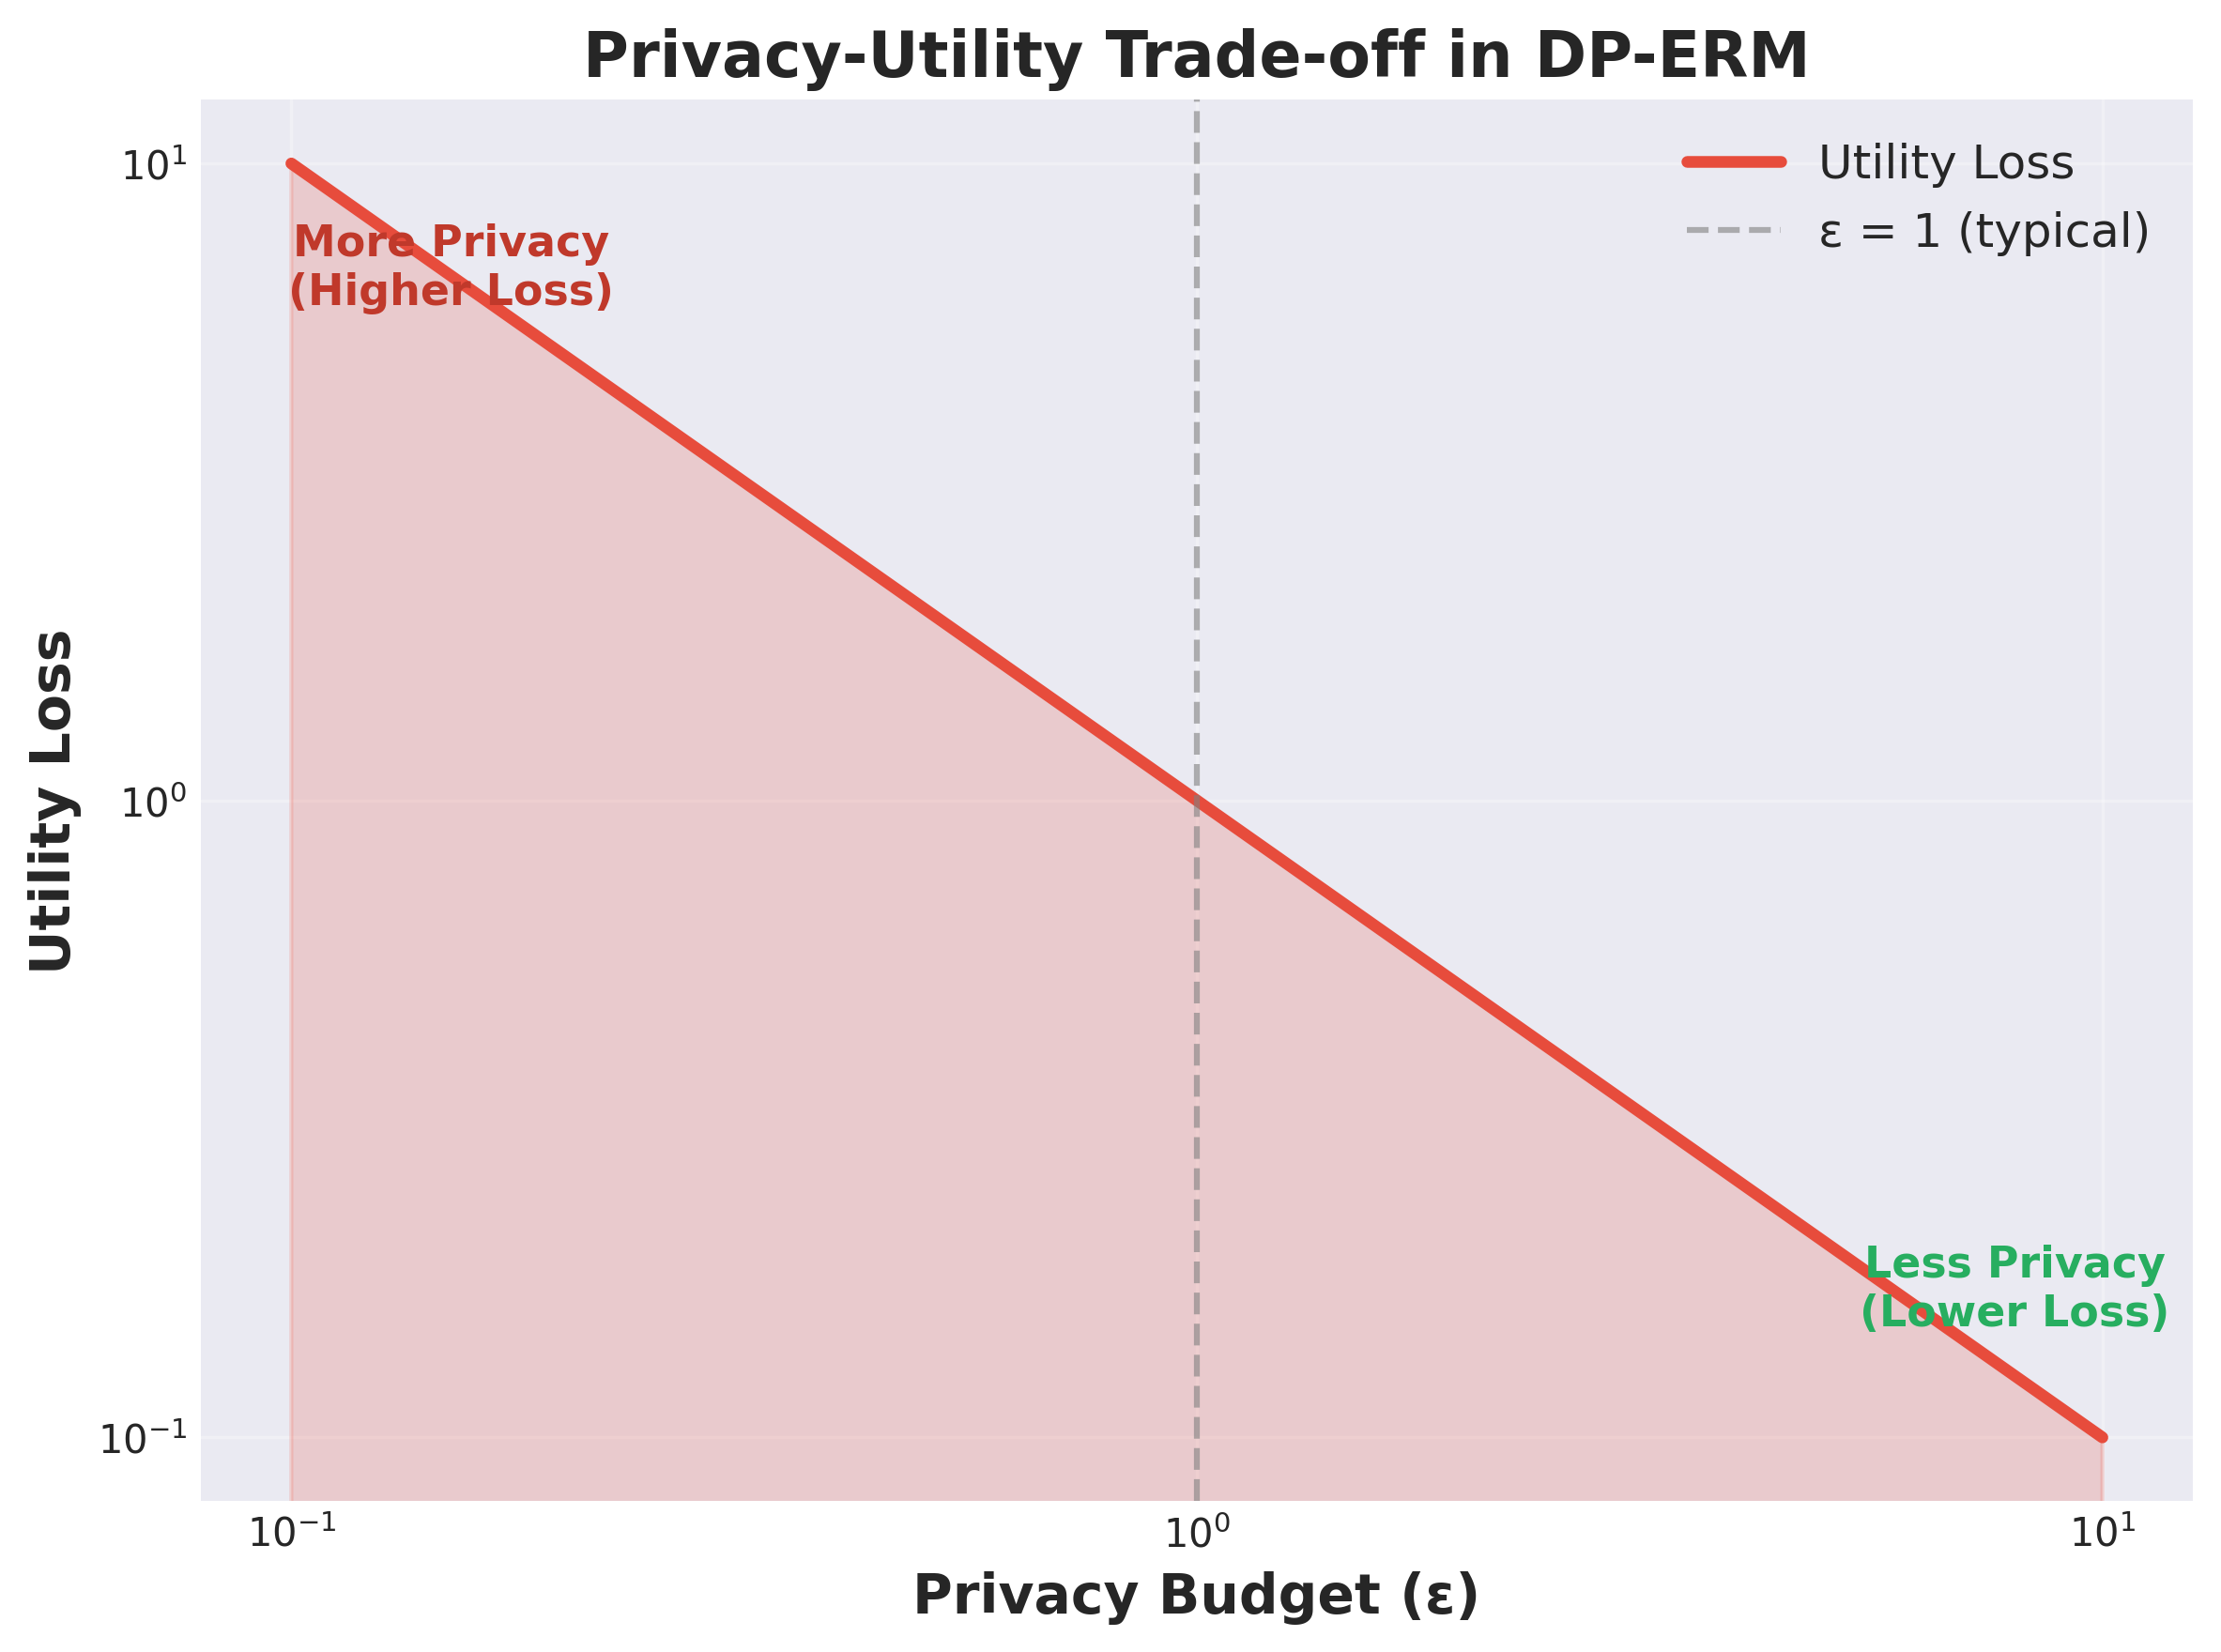
\includegraphics[width=0.9\textwidth]{privacy_tradeoff.png}
\end{center}
\vspace{0.5em}
\textbf{Differential Privacy (DP)} provides rigorous guarantees but at a cost...
\end{columns}

\vspace{0.5em}
\textbf{Course connection:} Fundamental privacy-utility trade-off from lecture
\end{frame}

\begin{frame}{The Curse of Dimensionality in DP-ERM}
\textbf{Standard Problem:}
\[
w^\star \in \arg\min_{w \in \mathbb{R}^p} \underbrace{\frac{1}{n} \sum_{i=1}^n \ell(w, d_i)}_{f(w)}
\]

\vspace{1em}
\textbf{Known Results (from course lower bounds lecture):}
\begin{itemize}
\item Bassily et al. (2014): DP-ERM utility degrades \alert{polynomially} with dimension $p$
\item For high-dimensional problems ($p \gg n$): \textbf{catastrophic utility loss}
\item Lower bound: $\Omega(\sqrt{p}/(n\varepsilon))$ for convex, $\ell_2$-bounded problems
\end{itemize}

\vspace{1em}
\begin{block}{The Challenge}
Can we achieve \alert{logarithmic} dependence on $p$ instead of polynomial?
\end{block}
\end{frame}

\begin{frame}{Prior Approaches and Limitations}
\begin{table}
\footnotesize
\begin{tabular}{@{}lll@{}}
\toprule
\textbf{Approach} & \textbf{Dimension Dependence} & \textbf{Limitation} \\
\midrule
DP-SGD & $\tilde{O}(p / n^{2/3})$ & Polynomial in $p$ \\
DP-Frank-Wolfe & $\tilde{O}(\log p / n^{2/3})$ & Requires $\ell_1$ constraint \\
Sparse regression & $\tilde{O}(\log p)$ & Needs known sparsity \\
Public data methods & $\tilde{O}(\log p)$ & Requires public data \\
\bottomrule
\end{tabular}
\end{table}

\vspace{1em}
\begin{alertblock}{Gap}
No algorithm achieves $\log p$ dependence for \emph{unconstrained} problems without prior structure knowledge
\end{alertblock}

\vspace{0.5em}
\textbf{Course connection:} Structure exploitation to beat worst-case bounds
\end{frame}

\section{Background}

\begin{frame}{Report-Noisy-Max: The Key Mechanism}
\textbf{Exponential Mechanism (from the course):}
\begin{itemize}
\item Utility function $u(x, y)$, sensitivity $\Delta_u$
\item Sample from $P(M(x) = y) \propto \exp(\varepsilon u(x,y)/(2\Delta_u))$
\end{itemize}

\vspace{0.8em}
\textbf{Report-Noisy-Max as Special Case:}
\begin{itemize}
\item Given scores $\{q_1, \ldots, q_p\}$: $\arg\max_j \{q_j + \text{Lap}(\Delta_j/\varepsilon)\}$
\item Reveals only \alert{1 index} instead of $p$ scalar values
\item \textbf{Exponential privacy savings compared to privatizing all $p$ values!}
\end{itemize}

\vspace{0.8em}
\textbf{Why this matters for DP-GCD:}
\begin{itemize}
\item DP-SGD: privatize all $p$ gradient coordinates $\Rightarrow$ noise $\propto \sqrt{p}$
\item DP-GCD: Report-Noisy-Max for coordinate selection + privatize only 1 coordinate
\item Noise scales as $\sqrt{T}$ not $\sqrt{p}$ when $T \ll p$: \textbf{massive savings}
\end{itemize}
\end{frame}

\begin{frame}{Coordinate Descent Basics}
\textbf{Standard Gradient Descent:}
\[
w_{t+1} = w_t - \alpha \nabla f(w_t) \quad \text{(update all $p$ coordinates)}
\]

\vspace{1em}
\textbf{Coordinate Descent:}
\[
w_{t+1} = w_t - \alpha_j [\nabla f(w_t)]_j \cdot e_j \quad \text{(update only coordinate $j$)}
\]

\vspace{1em}
\begin{columns}[T]
\column{0.5\textwidth}
\textbf{Random Selection}
\begin{itemize}
\item Pick $j$ uniformly at random
\item Simple, unbiased
\item May waste updates
\end{itemize}

\column{0.5\textwidth}
\textbf{Greedy Selection}
\begin{itemize}
\item Pick $j$ with largest $|\nabla_j f|$
\item Faster convergence
\item Exploits structure
\end{itemize}
\end{columns}

\vspace{0.5em}
\textbf{Course connection:} Optimization algorithms lecture (first-order methods)
\end{frame}

\section{The DP-GCD Algorithm}

\begin{frame}{Algorithm Overview}
\begin{algorithm}[H]
\caption{DP-GCD (Simplified)}
\footnotesize
\begin{algorithmic}[1]
\State \textbf{Input:} $w_0 \in \mathbb{R}^p$, iterations $T$, noise scales $\{\sigma_j, \sigma_j'\}$
\For{$t = 0$ to $T-1$}
    \State Compute gradient: $g = \nabla f(w_t)$
    \State \alert{Greedy selection (private):} 
    \[j_t \leftarrow \arg\max_{j \in [p]} \left\{ \frac{|g_j|}{\sqrt{M_j}} + \text{Lap}(\sigma_j) \right\}\]
    \State \alert{Noisy gradient coordinate:} $\tilde{g}_{j_t} \leftarrow g_{j_t} + \text{Lap}(\sigma_{j_t}')$
    \State \alert{Single coordinate update:} $w_{t+1} \leftarrow w_t - \gamma_{j_t} \tilde{g}_{j_t} e_{j_t}$
\EndFor
\State \textbf{Return} $w_T$
\end{algorithmic}
\end{algorithm}

\vspace{0.5em}
\textbf{Key idea:} Focus privacy budget on \emph{most informative} coordinates

\vspace{0.3em}
\textbf{Course connection:} Combining mechanism design with optimization
\end{frame}

\begin{frame}{Why Greedy Selection Helps Privacy}
\textbf{DP-SGD approach:}
\begin{itemize}
\item Privatize all $p$ gradient coordinates $\Rightarrow$ noise scales as $\sqrt{p}$
\item Wasted noise on irrelevant coordinates
\end{itemize}

\vspace{1em}
\textbf{DP-GCD approach:}
\begin{itemize}
\item \alert{Report-Noisy-Max}: Select coordinate privately (reveals only index)
\item Privatize only \alert{1 coordinate} per iteration
\item Noise scales as $\sqrt{T}$, not $\sqrt{p}$
\item When $T \ll p$: massive savings!
\end{itemize}

\vspace{1em}
\begin{block}{Intuition}
For sparse/quasi-sparse problems, only $s \ll p$ coordinates matter.\\
DP-GCD automatically finds and updates them.
\end{block}

\vspace{0.3em}
\textbf{Course connection:} Sensitivity analysis---coordinate-wise sensitivity $\Delta_1^j = 2L_j/n$ enables fine-grained noise
\end{frame}

\begin{frame}{Privacy Guarantees}
\begin{theorem}[Privacy (Theorem 4.2)]
With noise scales:
\[
\sigma_j = \sigma_j' = \frac{8L_j}{n} \sqrt{T \log(1/\delta)} / \varepsilon
\]
DP-GCD is $(\varepsilon, \delta)$-differentially private.
\end{theorem}

\vspace{0.5em}
\textbf{Proof sketch using course concepts:}
\begin{enumerate}
\item Each iteration: 2 data accesses (selection + gradient)
\item \textbf{Sensitivity:} Coordinate $j$ gradient has $\ell_1$-sensitivity $\Delta_1^j = 2L_j/n$
\item \textbf{Laplace mechanism:} Adding $\text{Lap}(\Delta_1^j/\varepsilon_t)$ gives $\varepsilon_t$-DP
\item \textbf{Advanced composition:} Over $2T$ mechanisms with $\varepsilon_t = \varepsilon/(2\sqrt{2T\log(1/\delta)})$ yields $(\varepsilon, \delta)$-DP
\end{enumerate}

\vspace{0.5em}
Solving for $\sigma_j$: $\sigma_j = \Delta_1^j/\varepsilon_t = \frac{2L_j}{n} \cdot \frac{2\sqrt{2T\log(1/\delta)}}{\varepsilon} = \frac{8L_j\sqrt{T\log(1/\delta)}}{n\varepsilon}$

\vspace{0.3em}
\textbf{Key insight:} Advanced composition theorem gives $\sqrt{T}$ dependence (basic composition would give linear $T$)
\end{frame}

\section{Theoretical Results}

\begin{frame}{Main Utility Results}
\begin{theorem}[Utility (Theorem 4.4, Simplified)]
Let $R_{M,1} = \|w_0 - w^\star\|_{M,1}$. With high probability:

\vspace{0.5em}
\textbf{Convex case:}
\[
f(w_\text{priv}) - f^\star = \tilde{O}\left( \frac{R_{M,1}^{4/3} L_{\max}^{2/3} \alert{\log^{1/3} p}}{n^{2/3}} \right)
\]

\textbf{Strongly convex case:}
\[
f(w_\text{priv}) - f^\star = \tilde{O}\left( \frac{L_{\max}^2 \alert{\log^2 p}}{\mu_{M,1} n^2} \right)
\]
\end{theorem}

\vspace{1em}
\begin{alertblock}{Key Achievement}
\alert{Logarithmic} dependence on $p$ (not polynomial!)
\end{alertblock}

\vspace{0.3em}
\textbf{Course connection:} Sample complexity---$n^{-2}$ rate matches non-private optimal (up to log factors)
\end{frame}

\begin{frame}{Proof Idea: Strongly Convex Case}
\textbf{Step 1: Noisy descent lemma}
\begin{itemize}
\item By smoothness: $f(w_{t+1}) \leq f(w_t) - \frac{1}{2M_j}|\nabla_j f(w_t)|^2 + \text{noise}^2$
\end{itemize}

\vspace{0.5em}
\textbf{Step 2: Greedy selection advantage}
\begin{itemize}
\item Greedy rule ensures: $\frac{1}{M_j}|\nabla_j f(w_t)|^2 \geq \frac{\|\nabla f(w_t)\|^2}{4\sum_j M_j} - O(\text{noise})$
\end{itemize}

\vspace{0.5em}
\textbf{Step 3: Strong convexity}
\begin{itemize}
\item $\|\nabla f(w_t)\|^2 \geq 2\mu_{M,1}(f(w_t) - f^\star)$
\end{itemize}

\vspace{0.5em}
\textbf{Step 4: Recursion}
\begin{itemize}
\item $f(w_{t+1}) - f^\star \leq \rho (f(w_t) - f^\star) + O(\sigma^2)$ where $\rho < 1$
\item After $T = O(\log(1/\rho))$ iterations: exponential convergence + noise accumulation
\item Balancing gives $\tilde{O}(L^2 \log^2 p / (\mu n^2))$
\end{itemize}

\vspace{0.3em}
\textbf{Course connection:} Contraction analysis from optimization lecture
\end{frame}

\begin{frame}{Comparison with Prior Work}
\begin{table}
\footnotesize
\begin{tabular}{@{}lccc@{}}
\toprule
\textbf{Algorithm} & \textbf{Convex} & \textbf{Strongly Convex} & \textbf{Constraint} \\
\midrule
DP-SGD & $\tilde{O}(p/n^{2/3})$ & $\tilde{O}(p/n^2)$ & None \\
DP-FW & $\tilde{O}(\log p/n^{2/3})$ & $\tilde{O}(\log p^{4/3}/n^{4/3})$ & $\ell_1$ ball \\
\rowcolor{yellow!30}
DP-GCD & $\tilde{O}(\log p/n^{2/3})$ & $\alert{\tilde{O}(\log p/n^2)}$ & \textbf{None} \\
\bottomrule
\end{tabular}
\end{table}

\vspace{1em}
\textbf{Breakthrough:}
\begin{itemize}
\item Matches DP-FW without $\ell_1$ constraint
\item \alert{First} to achieve $\tilde{O}(\log p / n^2)$ for strongly convex
\item Works on general unconstrained problems
\end{itemize}
\end{frame}

\begin{frame}{Adaptation to Quasi-Sparsity}
\begin{definition}[($\theta, \varepsilon$)-Quasi-Sparsity]
Vector $w$ is $(\theta, \varepsilon)$-quasi-sparse if at most $\theta$ entries exceed $\varepsilon$ in magnitude.
\end{definition}

\vspace{1em}
\begin{theorem}[Theorem 4.7, Simplified]
For strongly convex problems with quasi-sparse solution, if iterates remain $s$-sparse:
\[
f(w_T) - f^\star = \tilde{O}\left( \frac{L_{\max}^2 \alert{s^2} \log^2 p}{\mu n^2} \right)
\]
\end{theorem}

\vspace{1em}
\textbf{Impact:} Dimension dependence reduced from $p$ to $\alert{s^2 \log^2 p}$

\vspace{0.5em}
\textbf{Crucial:} DP-GCD adapts \emph{automatically} without knowing $s$ a priori!

\vspace{0.3em}
\textbf{Course connection:} Effective dimension vs ambient dimension (high-dim stats lecture)
\end{frame}

\begin{frame}{How DP-GCD Exploits Structure}
\begin{center}
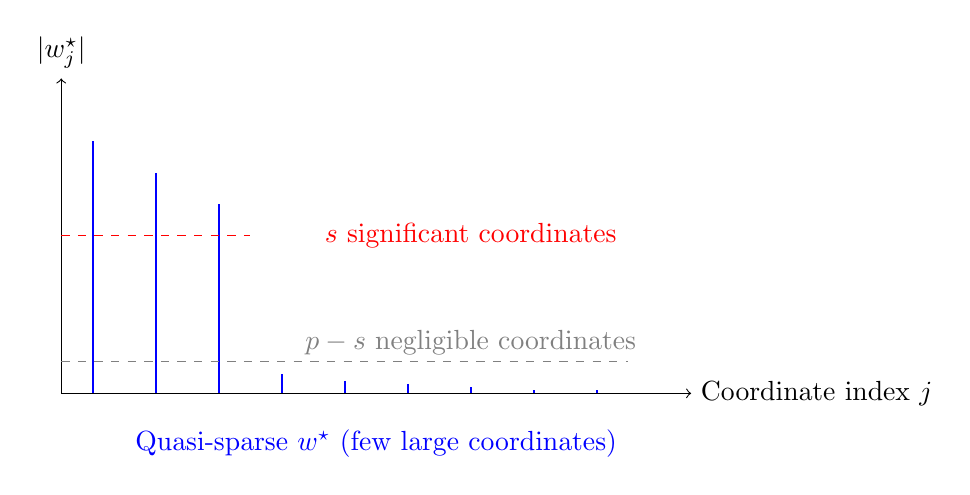
\begin{tikzpicture}[scale=0.8]
% Coordinate axis
\draw[->] (0,0) -- (10,0) node[right] {Coordinate index $j$};
\draw[->] (0,0) -- (0,5) node[above] {$|w_j^\star|$};

% Quasi-sparse solution
\draw[thick, blue] (0.5,4) -- (0.5,0);
\draw[thick, blue] (1.5,3.5) -- (1.5,0);
\draw[thick, blue] (2.5,3) -- (2.5,0);
\draw[thick, blue] (3.5,0.3) -- (3.5,0);
\draw[thick, blue] (4.5,0.2) -- (4.5,0);
\draw[thick, blue] (5.5,0.15) -- (5.5,0);
\draw[thick, blue] (6.5,0.1) -- (6.5,0);
\draw[thick, blue] (7.5,0.05) -- (7.5,0);
\draw[thick, blue] (8.5,0.05) -- (8.5,0);

\node[blue] at (5, -0.8) {Quasi-sparse $w^\star$ (few large coordinates)};

% Annotations
\draw[dashed, red] (0,2.5) -- (3,2.5);
\node[red] at (6.5, 2.5) {$s$ significant coordinates};
\draw[dashed, gray] (0,0.5) -- (9,0.5);
\node[gray] at (6.5, 0.8) {$p - s$ negligible coordinates};

\end{tikzpicture}
\end{center}

\textbf{DP-GCD behavior:}
\begin{itemize}
\item Greedy selection focuses on large coordinates early
\item Sparse iterates when initialized at $w_0 = 0$ (screening effect)
\item Converges in $T \approx s$ iterations (not $T \approx p$)
\end{itemize}
\end{frame}

\section{Experiments}

\begin{frame}{Experimental Setup}
\begin{table}
\scriptsize
\begin{tabular}{@{}lccl@{}}
\toprule
\textbf{Dataset} & $n$ & $p$ & \textbf{Notes} \\
\midrule
log1, log2 & 1,000 & 100 & Synthetic, quasi-sparse \\
square & 1,000 & 1,000 & Synthetic, 10 non-zeros \\
california & 20,640 & 8 & Real, low-dimensional \\
madelon & 2,600 & 501 & Real \\
dorothea & 800 & \alert{88,119} & Real, very high-dim \\
\bottomrule
\end{tabular}
\end{table}

\vspace{1em}
\textbf{Algorithms compared:}
\begin{itemize}
\item \textbf{DP-SGD:} Batch size 1, Gaussian noise
\item \textbf{DP-CD:} Random coordinate selection
\item \textbf{DP-GCD:} Greedy coordinate selection (proposed)
\end{itemize}

\vspace{0.5em}
\textbf{Privacy budget:} $\varepsilon = 1$, $\delta = 1/n^2$ (all experiments)

\vspace{0.5em}
\textbf{Metric:} Relative error $(f(w_t) - f^\star) / f^\star$ vs passes on data
\end{frame}

\begin{frame}{Key Experimental Results}
\begin{columns}[T]
\column{0.5\textwidth}
\textbf{High-dim sparse (dorothea)}
\begin{itemize}
\item DP-GCD: Only algorithm that \alert{converges}
\item DP-SGD/DP-CD: Cannot decrease objective
\item $p = 88k$: Dramatic advantage
\end{itemize}

\vspace{1em}
\textbf{Quasi-sparse (log2, madelon)}
\begin{itemize}
\item DP-GCD: $\sim 2$-$3\times$ faster convergence
\item Reaches $10^{-7}$ error vs $10^{-5}$ for baselines
\end{itemize}

\column{0.5\textwidth}
\textbf{Low-dimensional (california)}
\begin{itemize}
\item DP-GCD: Comparable to DP-SGD
\item Greedy overhead not justified
\item $p = 8$: No sparsity to exploit
\end{itemize}

\vspace{1em}
\textbf{Computational cost}
\begin{itemize}
\item 1 DP-GCD iter = full gradient
\item Equivalent to $p$ DP-CD iters
\item Justified by better utility per pass
\end{itemize}
\end{columns}

\vspace{1em}
\begin{alertblock}{Takeaway}
DP-GCD shines on high-dimensional problems with (quasi-)sparse structure
\end{alertblock}
\end{frame}

\begin{frame}{Visualization: log2 Results}
\begin{center}

\includegraphics[width=0.85\textwidth]{log2_results.png}
\end{center}

\vspace{-0.5em}
\scriptsize
\textbf{Observation:} DP-GCD (blue) converges much faster than DP-CD (red) and DP-SGD (green) on quasi-sparse logistic regression problem.
\end{frame}

\section{Critical Analysis}

\begin{frame}{Strengths}
\begin{enumerate}
\item \textbf{No domain constraints}
\begin{itemize}
\item Works on unconstrained problems (unlike DP-Frank-Wolfe)
\end{itemize}

\item \textbf{Automatic adaptation}
\begin{itemize}
\item Exploits quasi-sparsity without prior knowledge of $s$ or $\theta$
\end{itemize}

\item \textbf{Logarithmic dimension dependence}
\begin{itemize}
\item Achieves $\tilde{O}(\log p)$ in favorable settings
\end{itemize}

\item \textbf{Coordinate-wise adaptivity}
\begin{itemize}
\item Uses fine-grained Lipschitz constants $L_j$ for noise calibration
\end{itemize}

\item \textbf{First optimal strongly-convex rates}
\begin{itemize}
\item $\tilde{O}(\log p / n^2)$ without reduction tricks
\end{itemize}

\item \textbf{Strong empirical validation}
\begin{itemize}
\item Dramatic improvements on dorothea ($p = 88k$)
\end{itemize}
\end{enumerate}
\end{frame}

\begin{frame}{Limitations}
\begin{enumerate}
\item \textbf{Computational cost}
\begin{itemize}
\item Full gradient per iteration: $O(np)$ cost
\item Wall-clock time can be higher than randomized methods
\item Only justified when utility per pass matters more than time
\end{itemize}

\item \textbf{Proximal extension lacks theory}
\begin{itemize}
\item Proposes proximal variant for $\ell_1$ regularization
\item \alert{No utility analysis provided}
\item Greedy proximal CD is challenging even without privacy
\end{itemize}

\item \textbf{Assumption requirements}
\begin{itemize}
\item Needs coordinate-wise smoothness/Lipschitzness constants
\item Lower bound on initial gap: $f(w_0) - f^\star \geq \Omega(\cdots)$
\end{itemize}

\item \textbf{Not optimal in all regimes}
\begin{itemize}
\item When $\ell_2$-norm quantities bounded: doesn't match DP-SGD
\item Interpolates but doesn't dominate everywhere
\end{itemize}
\end{enumerate}
\end{frame}

\begin{frame}{Limitations (continued)}
\begin{enumerate}
\setcounter{enumi}{4}
\item \textbf{Privacy budget overhead}
\begin{itemize}
\item Report-Noisy-Max adds noise for coordinate selection
\item In low-dim: overhead outweighs benefits
\end{itemize}

\item \textbf{Limited to smooth objectives}
\begin{itemize}
\item Main theory assumes smooth losses
\item Extensions to non-smooth/constrained settings remain open
\end{itemize}

\item \textbf{Gap between theory and practice}
\begin{itemize}
\item Theoretical noise scales may be too conservative
\item Experiments use tuned hyperparameters (not theoretical formulas)
\end{itemize}
\end{enumerate}

\vspace{1em}
\begin{block}{When to Use DP-GCD}
High-dimensional problems with suspected quasi-sparsity where privacy-utility trade-off matters more than wall-clock time.
\end{block}
\end{frame}

\section{Conclusion}

\begin{frame}{Summary}
\textbf{Main Contributions:}
\begin{enumerate}
\item \textbf{DP-GCD algorithm:} Greedy coordinate descent with Report-Noisy-Max
\item \textbf{Theoretical guarantees:} $\tilde{O}(\log p)$ utility for unconstrained problems
\item \textbf{Automatic adaptation:} Exploits quasi-sparsity without prior knowledge
\item \textbf{Empirical validation:} Dramatic improvements on high-dim sparse problems
\end{enumerate}

\vspace{1em}
\textbf{Key Insight:}
\begin{block}{}
By focusing privacy budget on \alert{most informative} coordinates, DP-GCD achieves logarithmic dimension dependence and automatically adapts to problem structure.
\end{block}

\vspace{1em}
\textbf{Impact:} Opens door to practical private learning in high dimensions (genomics, NLP, high-dim regression).
\end{frame}

\begin{frame}{Open Questions}
\begin{enumerate}
\item \textbf{Proximal analysis:} Can we rigorously analyze the proximal variant for non-smooth regularizers?

\item \textbf{Optimal algorithm:} Does there exist an algorithm achieving optimal utility in \emph{all} regimes (both $\ell_1$ and $\ell_2$ bounded)?

\item \textbf{Computational efficiency:} Can we reduce per-iteration cost while preserving privacy-utility benefits?

\item \textbf{Extensions:} How does DP-GCD perform on non-convex problems (neural networks)?

\item \textbf{Fairness implications:} Does sparsity exploitation introduce fairness concerns (favoring represented groups)?
\end{enumerate}

\vspace{1em}
\begin{alertblock}{Research Direction}
Toward adaptive DP algorithms that automatically exploit problem structure without sacrificing worst-case guarantees.
\end{alertblock}
\end{frame}

\begin{frame}[standout]
\Huge Thank You!
\vspace{2em}

\normalsize
Questions?

\vspace{2em}
\footnotesize
\textit{Mangold, P., Bellet, A., Salmon, J., and Tommasi, M.\\
High-Dimensional Private Empirical Risk Minimization\\
by Greedy Coordinate Descent. AISTATS 2023.}
\end{frame}

\appendix

\begin{frame}[allowframebreaks]{Backup: Technical Details}
\textbf{Coordinate-wise Regularity Assumptions}

\vspace{0.5em}
\textbf{Component smoothness:}
\[
f(w) \leq f(v) + \langle \nabla f(v), w - v \rangle + \frac{1}{2} \|w - v\|_{M,2}^2
\]
where $\|w\|_{M,2}^2 = \sum_{j=1}^p M_j w_j^2$.

\vspace{0.5em}
\textbf{Component Lipschitzness:} For each $j$,
\[
|f(w + t e_j) - f(w)| \leq L_j |t|
\]

\vspace{0.5em}
\textbf{Strong convexity w.r.t. $\ell_1$ norm:}
\[
f(w) \geq f(v) + \langle \nabla f(v), w - v \rangle + \frac{\mu_{M,1}}{2} \|w - v\|_{M,1}^2
\]

\framebreak

\textbf{Report-Noisy-Max Mechanism}

\vspace{0.5em}
Given scores $\{q_1, \ldots, q_p\}$ with coordinate-wise $\ell_1$-sensitivities $\{\Delta_1, \ldots, \Delta_p\}$:
\[
j^\star = \arg\max_{j \in [p]} \{q_j + \text{Lap}(\Delta_j / \varepsilon)\}
\]

\textbf{Privacy guarantee:} $\varepsilon$-DP (pure)

\textbf{Why it's powerful:} Reveals only the index (1 number), not all $p$ scores.

\textbf{Connection to exponential mechanism:} This is a special case where utility function $u(D, j) = q_j$ has sensitivity $\Delta_j$.

\framebreak

\textbf{Proof Sketch: Utility Bound (Convex Case)}

\vspace{0.5em}
\textbf{Noisy descent lemma:}
\[
f(w_{t+1}) - f(w_t) \leq -\frac{1}{2M_j} |\nabla_j f(w_t)|^2 + \text{noise terms}
\]

\vspace{0.5em}
\textbf{Key property:} Greedy selection ensures
\[
\frac{1}{M_j} |\nabla_j f(w_t)|^2 \geq \frac{\|\nabla f(w_t)\|^2}{2 \sum_j M_j}
\]

\vspace{0.5em}
Either:
\begin{itemize}
\item $w_t$ far from optimum $\Rightarrow$ progress despite noise
\item $w_t$ close to optimum $\Rightarrow$ remain in small ball
\end{itemize}

Balancing these two regimes + Chernoff bounds gives the result.

\framebreak

\textbf{Advanced Composition and RDP}

\vspace{0.5em}
\textbf{Classical Advanced Composition} (Theorem 3.20 in Dwork \& Roth):
\[
\varepsilon = \sqrt{2k\log(1/\delta)} \cdot \varepsilon_0 + k\varepsilon_0^2
\]

\vspace{0.5em}
\textbf{Renyi Differential Privacy (from the course):}
\begin{itemize}
\item Renyi divergence: $D_\alpha(p\|q) = \frac{1}{\alpha-1}\log \mathbb{E}_{Y \sim q}[(p(Y)/q(Y))^\alpha]$
\item $(\alpha, \rho)$-RDP if $D_\alpha(p_{x}\|p_{x'}) \leq \rho$ for all neighboring $x, x'$
\item \textbf{Composition:} $(\alpha, \rho_1)$-RDP + $(\alpha, \rho_2)$-RDP $\Rightarrow$ $(\alpha, \rho_1 + \rho_2)$-RDP
\item \textbf{Conversion:} $(\alpha, \rho)$-RDP $\Rightarrow$ $(\rho + \log(1/\delta)/(\alpha-1), \delta)$-DP
\end{itemize}

\vspace{0.5em}
\textbf{Why this matters for DP-GCD:}
\begin{itemize}
\item $2T$ data accesses, advanced composition gives $\sqrt{T}$ (not linear $T$)
\item Enables practical privacy budgets: $\sigma \propto \sqrt{T}$ vs $\sigma \propto T$
\end{itemize}
\end{frame}

\begin{frame}{Backup: Synthetic Data Generation}
\textbf{log1 / log2:}
\begin{itemize}
\item $X \in \mathbb{R}^{1000 \times 100}$, columns $\sim \mathcal{N}(0, 1)$
\item $w_{\text{true}} \sim \text{LogNormal}(0, \sigma)$ with $\sigma \in \{1, 2\}$
\item For logistic: $y_i \sim \text{Bernoulli}(\sigma(x_i^\top w_{\text{true}} + \xi_i))$
\item LogNormal creates quasi-sparsity (few large values, many small)
\end{itemize}

\vspace{1em}
\textbf{square:}
\begin{itemize}
\item $X \in \mathbb{R}^{1000 \times 1000}$, columns $\sim \mathcal{N}(0, 1)$
\item $w_{\text{true}}$ has exactly 10 non-zero entries (chosen at random)
\item $y = X w_{\text{true}} + \xi$ with $\xi \sim \mathcal{N}(0, \sigma^2)$
\item Used with squared loss + $\ell_1$ regularization (LASSO)
\end{itemize}
\end{frame}

\begin{frame}{Backup: Q\&A Preparation}
\textbf{Expected Questions:}

\vspace{0.5em}
\textbf{Q1: Why does greedy selection help with privacy?}\\
A: Report-Noisy-Max reveals only 1 index (not $p$ values), exponential privacy savings. Noise scales as $\sqrt{T}$ not $\sqrt{p}$.

\vspace{0.5em}
\textbf{Q2: What if solution isn't sparse?}\\
A: Algorithm interpolates between $\log p$ and $p$ dependence based on actual structure. Utility naturally depends on $\ell_1$-norm quantities.

\vspace{0.5em}
\textbf{Q3: Computational cost seems high?}\\
A: Yes, but justified when dimensionality (not time) is the bottleneck. For high-dim sparse problems, achieves better utility per data pass.

\vspace{0.5em}
\textbf{Q4: Fairness implications?}\\
A: Open question! Quasi-sparsity exploitation might favor well-represented groups. If features correlate with protected attributes, greedy selection could amplify bias.

\vspace{0.5em}
\textbf{Q5: Connection to course on group privacy?}\\
A: Could extend DP-GCD to protect feature groups by modifying sensitivity calculations and greedy selection rule.
\end{frame}

\end{document}
